\chapter{Software as a Service}

\section{Cloud Computing}
La differenza tra il possedere e l'utilizzare. E' questo l'aspetto cruciale del cambiamento apportato dal cloud computing rispetto al software tradizionale. Le risorse, che siano esse stesse archiviazione, elaborazione o qualsivoglia risorsa informatica, non sono mai ad hoc per un singolo utente, ma vengono assegnate on demand ai singoli utenti e appartengono ad un insieme condiviso da tutti gli altri utenti del prodotto utenti. Attraverso internet ogni utente può accedere a queste risorse in qualsiasi momento. Tali risorse vengono opportunamente allocate all'utente in maniera dinamica e completamente automatizzata. L'utente può utilizzare così anche software non installati sul proprio computer o usufruire di una memoria di massa accessibile da parte sua da qualsiasi dispositivo.
\paragraph{}
L'esperienza utente che si vuole fornire però è quella di un utilizzo esclusivo della risorsa, come nei software tradizionali, quando in realtà la risorsa viene solo sapientemente distribuita tra gli utenti. Ciò fa si che, potenzialmente, un singolo utente possa acquisire risorse notevolmente maggiori nel caso medio
\begin{figure}
	\centering
	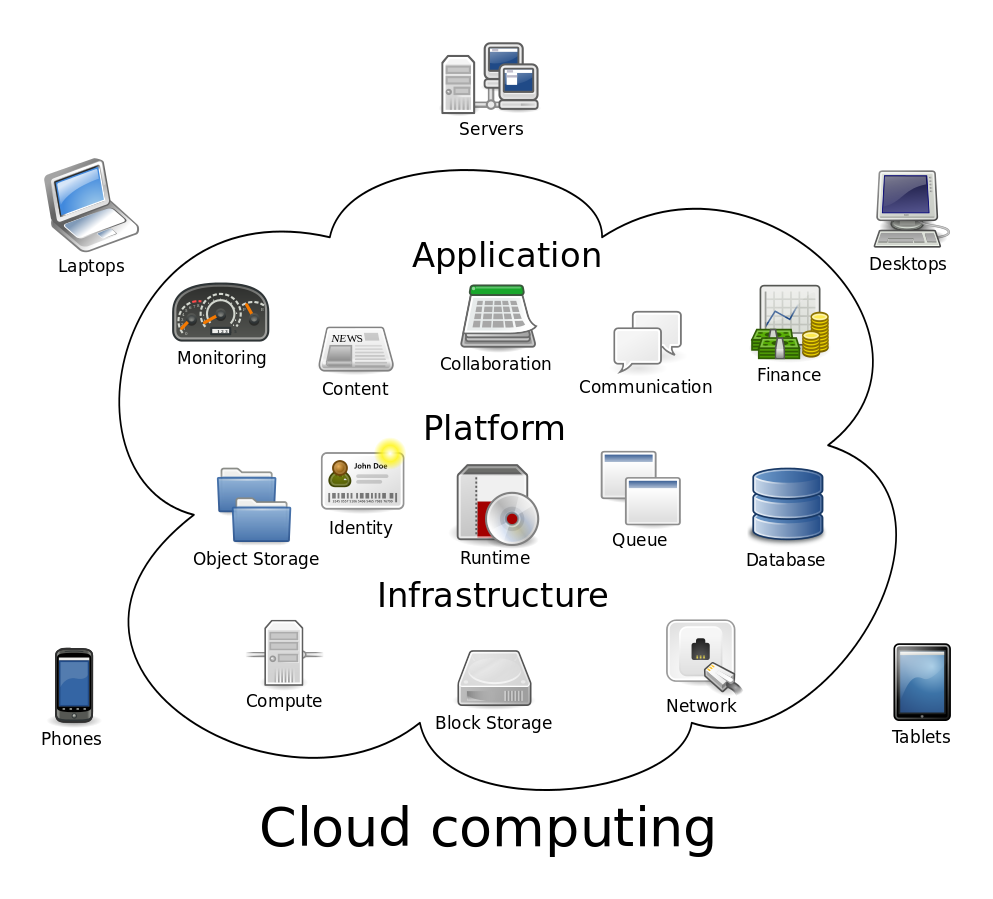
\includegraphics[width=0.7\linewidth]{capitoli/imgs/CloudComputing}
	\caption{Diagramma logico di una rete Cloud Computing}
	\label{fig:cloudcomputing}
\end{figure}
\subsection{Vantaggi del Cloud Computing}
\begin{itemize}
	\item Costo: \\
	Con l'avvento del cloud tutta la gestione dell'infrastruttura sottostante il software diviene a carico del provider. Vengono eliminate spese per la gestione dei data center locali. Facendo riferimento alla versione SaaS di BigFix ad esempio, il cliente viene sollevando dal pesante onere di utilizzare server locali e gestirne le relative connessioni. Il provider detiene tutto l'hardware di cui il cliente ha bisogno.
	
	\item Velocità: \\
	Anche quì ci risulta molto utile prendere ad esempio la suite di BigFix. quando un nuovo cliente acquista il prodotto nella sua versione on-premises, un'incaricato di IBM si reca presso il cliente e lì inizia un lungo processo di installazione della suite che può impiegare diverse ore. nella scenario SaaS il cambiamento è radicale. E' sufficente che il cliente compili una form online, dopo alcuni minuti poi riceve una mail con il link per accedere al servizio.
	
	\item Prestazioni \\
	Una delle motivazioni principali per la quale si sceglie di fare uso del clud computing sono proprio le prestazioni, soprattutto secondo il paradigma PaaS. Esternalizzando le risorse di calcolo, si può fare affidamento a dei provider che fanno dei server ad alte prestazioni il loro punto di forza. L'utente può in questo modo abbattere dei bottleneck che altrimenti risulterebbero di grande impedimento. Nel 2016 IBM mette per la prima volta a disposizione pubblicamente un computer quantico, proprio attraverso una piattaforma cloud (IBM Q). Questo può rappresentare un esempio estremo in ottica prestazioni, ma che può rendere un'idea di quale potrà essere il trend nei prossimi.
	
	\item Affidabilità \\
	Operazioni di mirroring da parte dei provider dei servizi cloud fa sì che il backup dei dati sia continuo ed economico.
\end{itemize}

\section{Tipologie di servizi Cloud}
Il termine Cloud risulta in realtà molto generico. Esso comprende diverse tipologie di fornitura dei servizi, a seconda della risorsa che viene offerta dal provider. La maggior parte dei servizi di Cloud Computing rientrano in tre tipologie principali: Infrastruttura distribuita come Servizio (IaaS, Infrastructure as a Service), Piattaforma distribuita come Servizio (PaaS, Platform as a Service) e Software come un Servizio (SaaS, Software as a Service). Oltre a queste tipologie, annoveriamo anche soluzioni minori come il DaaS (Data a a Service) e l'HaaS (Hardware as a Service). Andiamo a vedere nel dettaglio come, a seconda della modalità di utilizzo del paradigma Cloud, queste tipologie si differenziano. 
\begin{figure}
	\centering
	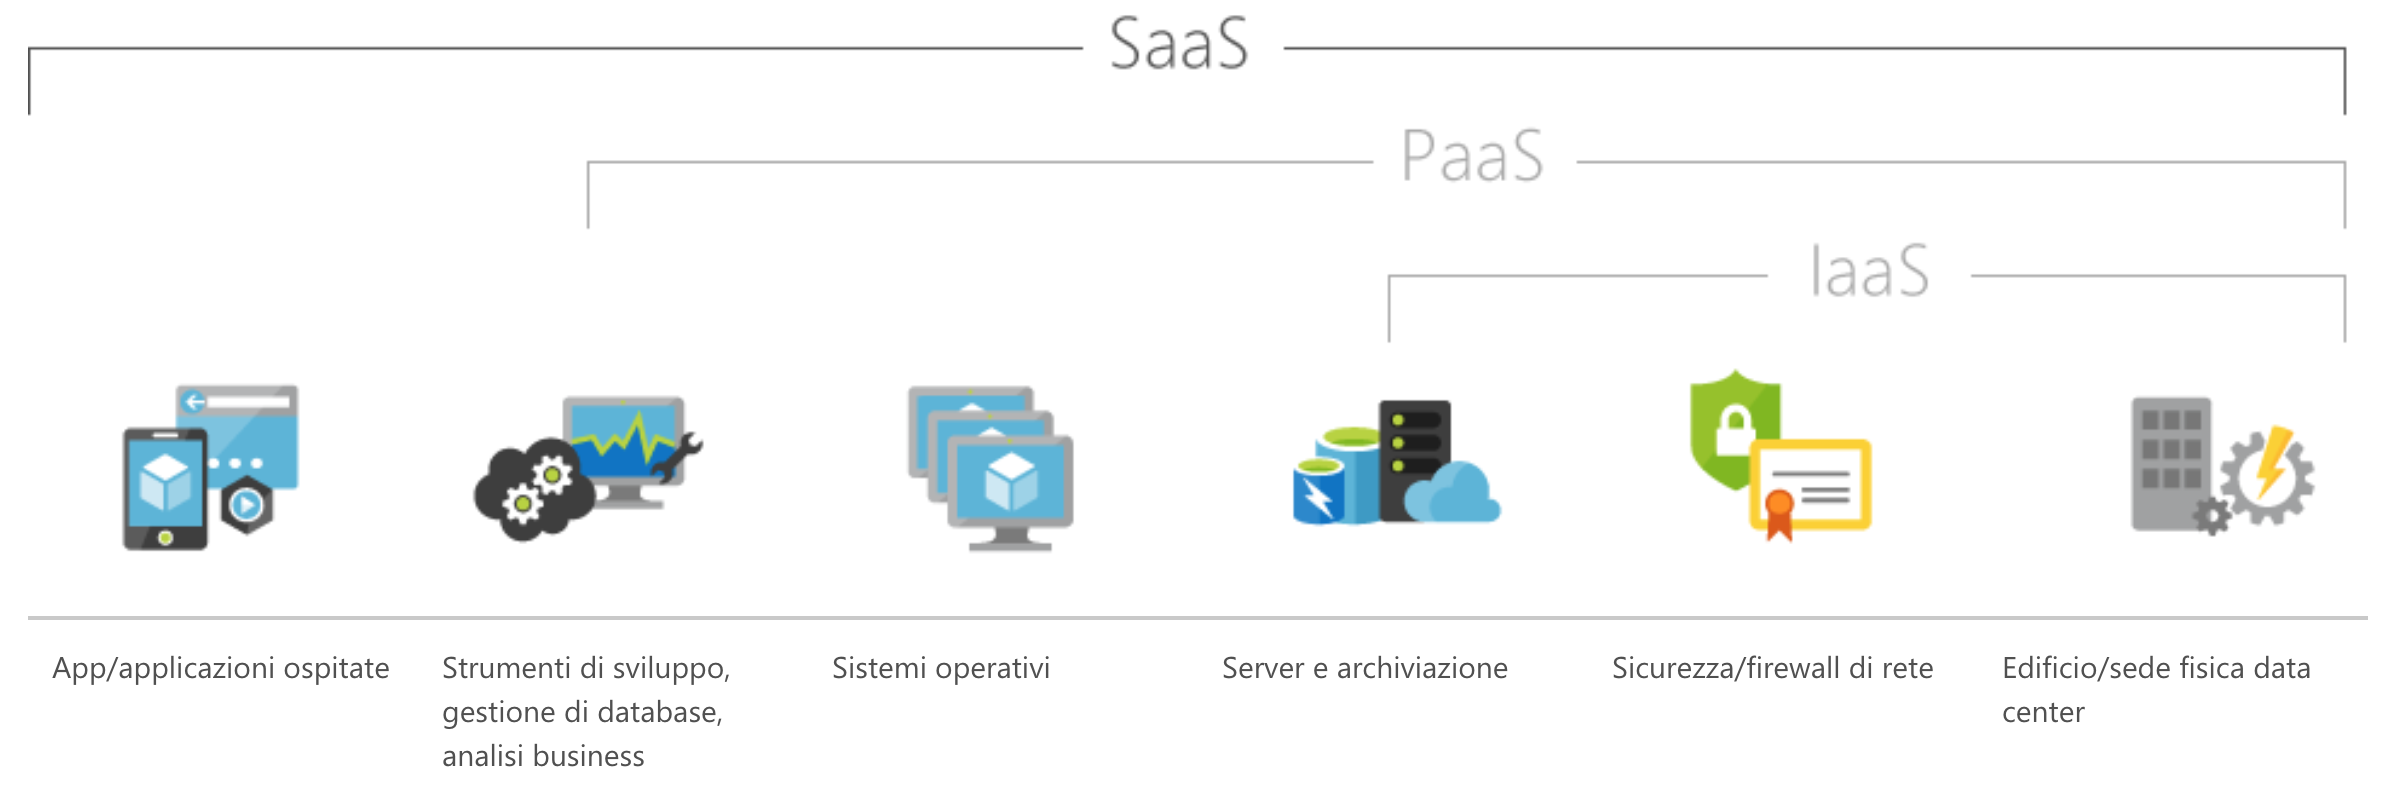
\includegraphics[width=0.7\linewidth]{capitoli/imgs/TipologieCloud}
	\caption{Panoramica delle principali tipologie Cloud}
	\label{fig:tipologiecloud}
\end{figure}

\subsection{IaaS, Infrastructure as a Service}
E' la tipologia più basilare. Vengono messe a disposizione piattaforme di elaborazione. Utilizzando un IaaS si affittano le infrastrutture utili ai propri scopi, come add esempio server, macchine virtuali (VMs), risorse di archiviazione, reti e sistemi operativi. Può, inoltre, essere messo a isposizione anche hardware in remoto. Il provider di servizi cloud gestisce l'infrastruttura, mentre l'utente acquista, installa, configura e gestisce il software, tra cui sistemi operativi, middleware e applicazioni.
\subsection{PaaS, Platform as a Service}
Una piattaforma distribuita come servizio (PaaS, Platform as a Service) è un ambiente cloud di sviluppo completo. Una soluzione PaaS è progettata per consentire il ciclo completo dello sviluppo delle applicazioni: creazione, test, distribuzione, gestione e aggiornamento. L'utente ha tutta la libertà di sviluppare gli applicativi a proprio piacimento, ma lavora con componenti software già pronti all'utilizzo (microservices). Questi componenti non sono localizzati presso chi utilizza il cloud, bensì presso il provider, il quale si occupa del loro mantenimento e aggiornamento. 
\subsubsection{IBM Bluemix}
Troviamo, sempre all'interno di IBM, uno dei principali servizi cloud PaaS presenti sul mercato: IBM BlueMix. L'utente può usufruire di un'astrazione di molte componenti utili allo sviluppo. Si può, ad esempio, fare uso di Database specifici o moduli dedicati all'IoT. Ne vediamo alcuni esempi nella figura 3.3
\begin{figure}
	\centering
	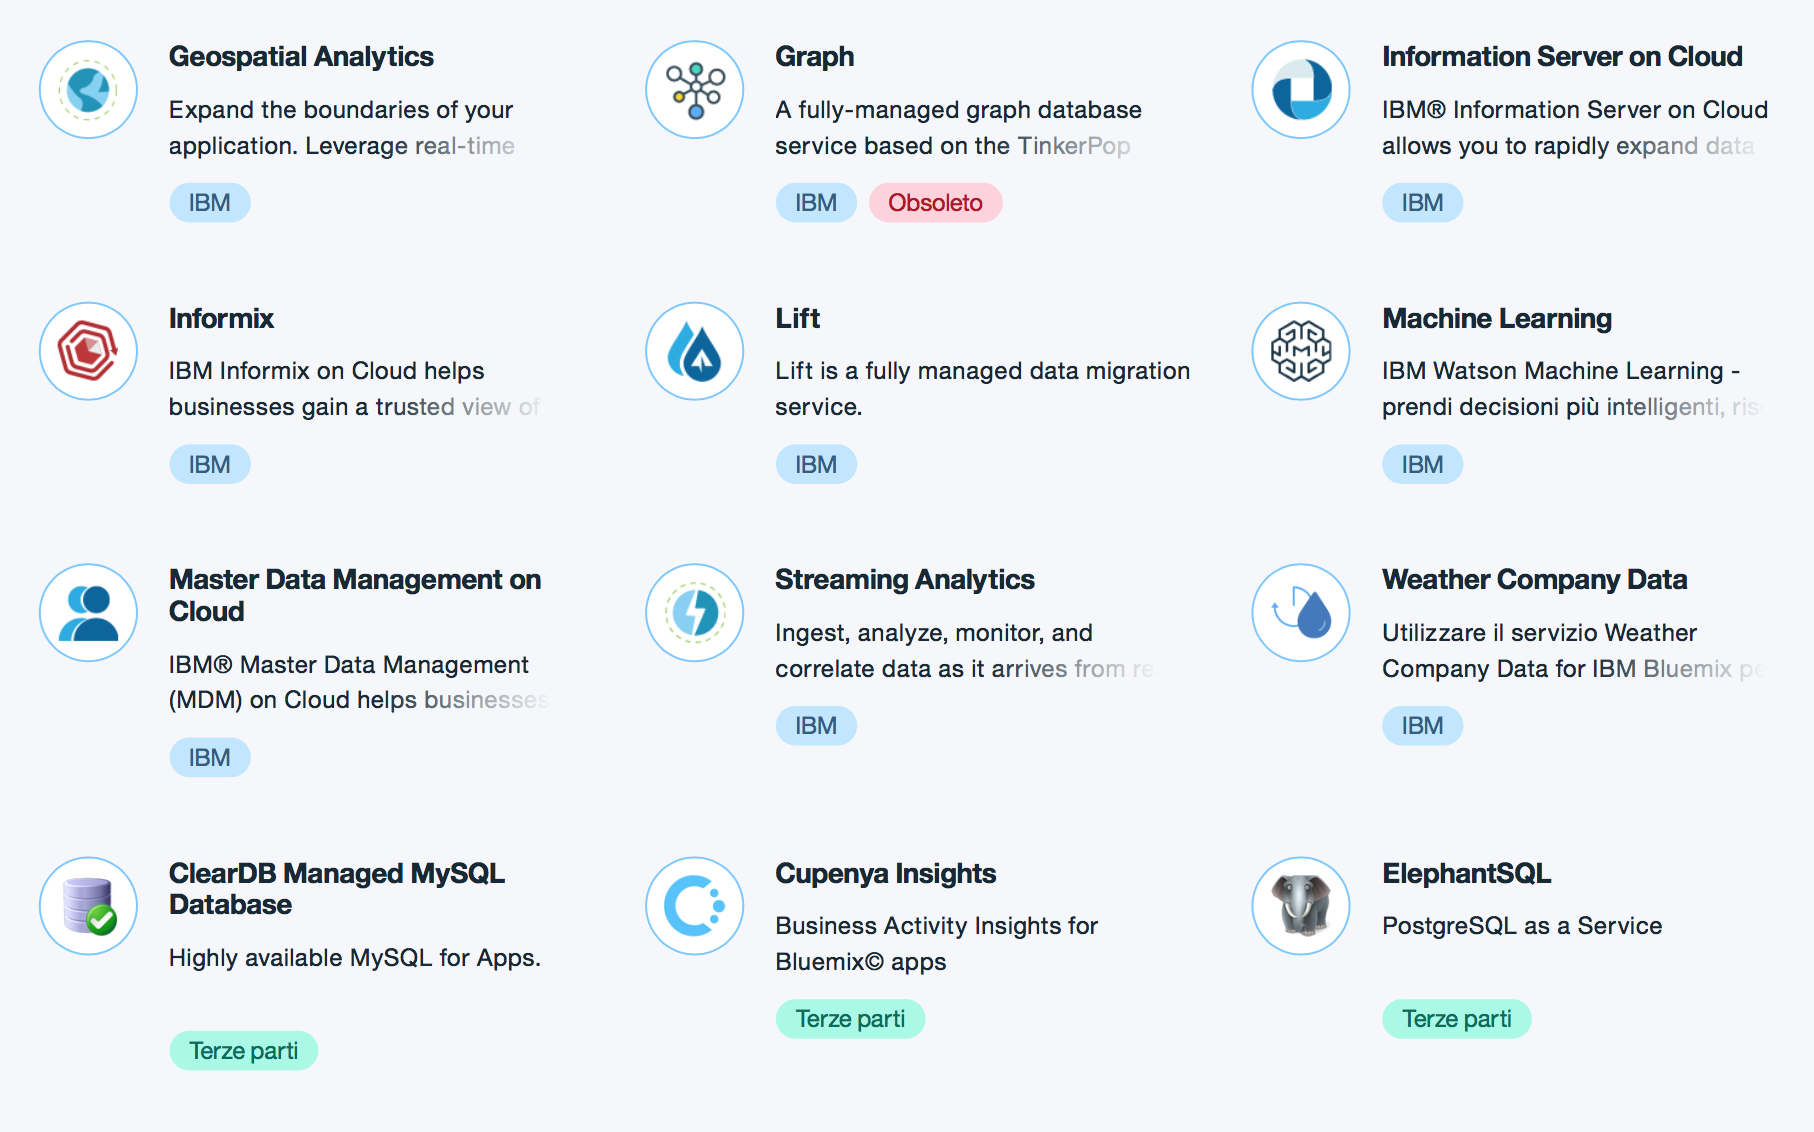
\includegraphics[width=0.7\linewidth]{capitoli/imgs/catalog}
	\caption{Alcuni esempi di moduli presenti nel catalogo BlueMix}
	\label{fig:catalog}
\end{figure}
\paragraph{IBM Watson}
Tra le componenti sviluppate da IBM merita una menzione anche Watson. Watson è un sistema di intelligenza artificiale in grado di rispondere a domande espresse in un linguaggio naturale. Tra le funzionalità ricordiamo quelle di elaborazione del linguaggio naturale, information retrieval, rappresentazione della conoscenza, ragionamento automatico e tecnologie di apprendimento automatico.
\begin{figure}
	\centering
	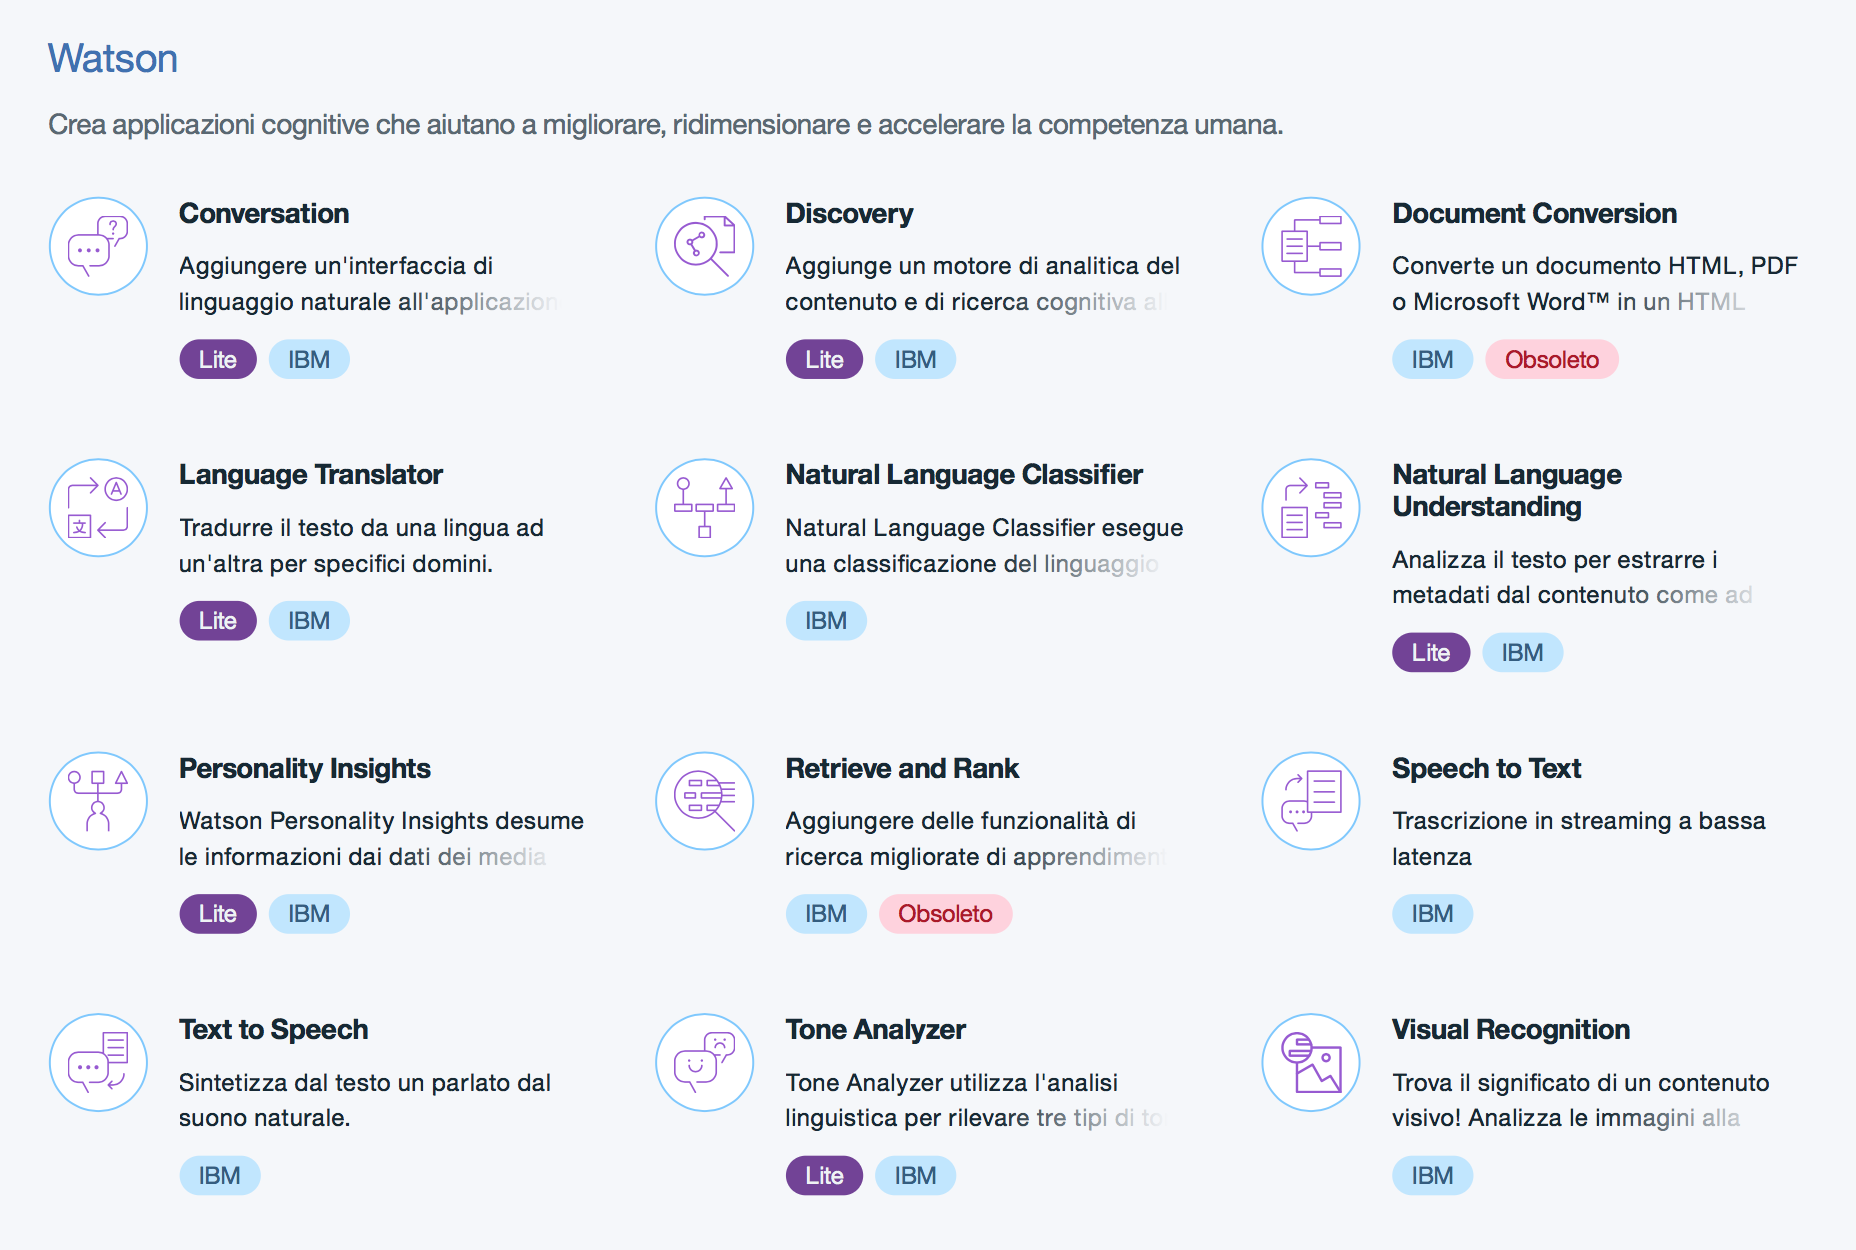
\includegraphics[width=0.7\linewidth]{capitoli/imgs/watson}
	\caption{Alcuni moduli appartenenti a Watson}
	\label{fig:watson}
\end{figure}


\subsection{SaaS, Software as a Service}

\section{Confronto tra SaaS e On Premise}
\paragraph{Vantaggi del Software On Premise}
\begin{itemize}
	\item  Controllo esclusivo su sistemi e dati
	\item Gestione interna dei dati sensibili
	\item Alto investimento iniziale ammortizzato nel lungo periodo
\end{itemize}

\paragraph{}
Il paradigma di fornitura on premise risulta ancora essere la soluzione più adatta nel caso in cui la gestione diretta dei dati sia fondamentale per policy aziendali oppure sia necessaria una maggiore flessibilità di configurazione per l’integrazione con altre architetture software. Un'altro requisito è che l'architettura fisica del software sia geograficamente localizzata.
